\subsection{Einregeln der optimalen Verzögerungszeit}
\input{tabelleverzögerung.tex}
\begin{figure}[h!]
  \centering
  \includegraphics[width=\textwidth]{figverzögerung.pdf}
  \caption{Optimierung der Verzögerungszeit: Verzögerungszeit $T_{\text{VZ}}$ gegen Spannungsimpuls $U$}
  \label{fig:verzögerung}
\end{figure}
Fit
\begin{equation*}
  N = -a \left( T_{\text{VZ}} +b \right)^4+c
\end{equation*}
Fitparameter
\begin{align*}
  a &=& \SI{4.82149138 \pm 0.236142743e-04}{}\\
  b &=& \SI{2.08543593 \pm 0.229205656}{}\\
  c &=& \SI{208.001211 \pm 3.50366199}{}\\
\end{align*}

\FloatBarrier
\subsection{Kalibrierung des Multi-Channel-Analysers}
\begin{table}[h!]
  \centering
  \caption{Messdaten zu Kalibrierung des Multi-Channel-Analysers}
  \label{tab:kalibrierung}
  \begin{tabular}{c c c c}
    \toprule
%    \multicolumn{3}{c}{$f_{\text{1, theo}}=\SI{0.1}{m}$} & \multicolumn{3}{c}{$f_{\text{2, theo}}=\SI{0.05}{m}$}\\
      Channel & $\Delta$ t $/ 10^{-6} s$ & Channel & $\Delta$ t $/ 10^{-6} s$ \\
      \midrule
         24   &   1407  &  247   &   1680 \\
         46   &   1561  &  270   &   1555 \\
         69   &   1400  &  292   &   1608 \\
         91   &   1294  &  315   &   1384 \\
        113   &   1298  &  337   &   1952 \\
        136   &   1034  &  359   &   1880 \\
        158   &   1502  &  382   &   2008 \\
        180   &   1336  &  404   &   2088 \\
        203   &   1700  &  427   &   2024 \\
        225   &   1644  &  445   &   3384 \\
    \bottomrule
  \end{tabular}
\end{table}

%\end{landscape}
%\end{document}

\begin{figure}[h!]
  \centering
  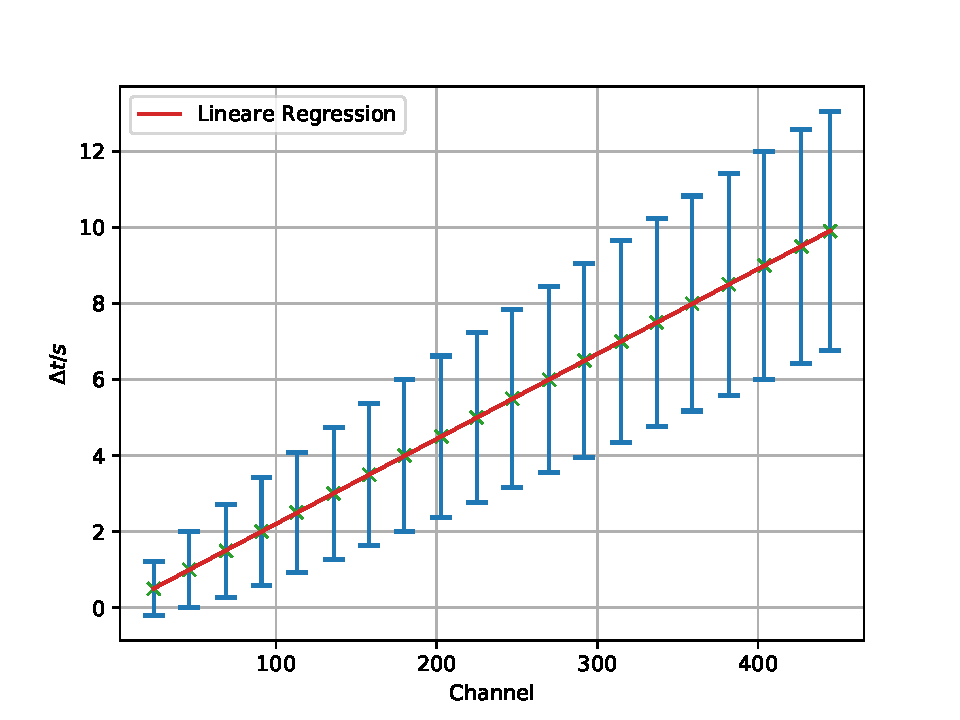
\includegraphics[width=\textwidth]{figkalibrierung.pdf}
  \caption{Kalibrierung des Multi-Channel-Analysers: Zeitlicher Abstand des Doppelimpulses $\Delta$ t gegen den zugehörigen Channel}
  \label{fig:kalibrierung}
\end{figure}
Fit: C $\widehat{=}$ Channel
\begin{equation*}
\Delta t = a \cdot C + b
\end{equation*}
Fitparameter:
\begin{align*}
a  &=&  \SI{ 0.02234091 \pm 1.28401231692e-05}{\frac{1}{s}}  \\
b  &=&  \SI{-0.03080493 \pm 0.00345318109864 }{}  \\
\end{align*}

\FloatBarrier

\subsection{Messung der Lebensdauer}
\begin{figure}[h!]
  \centering
  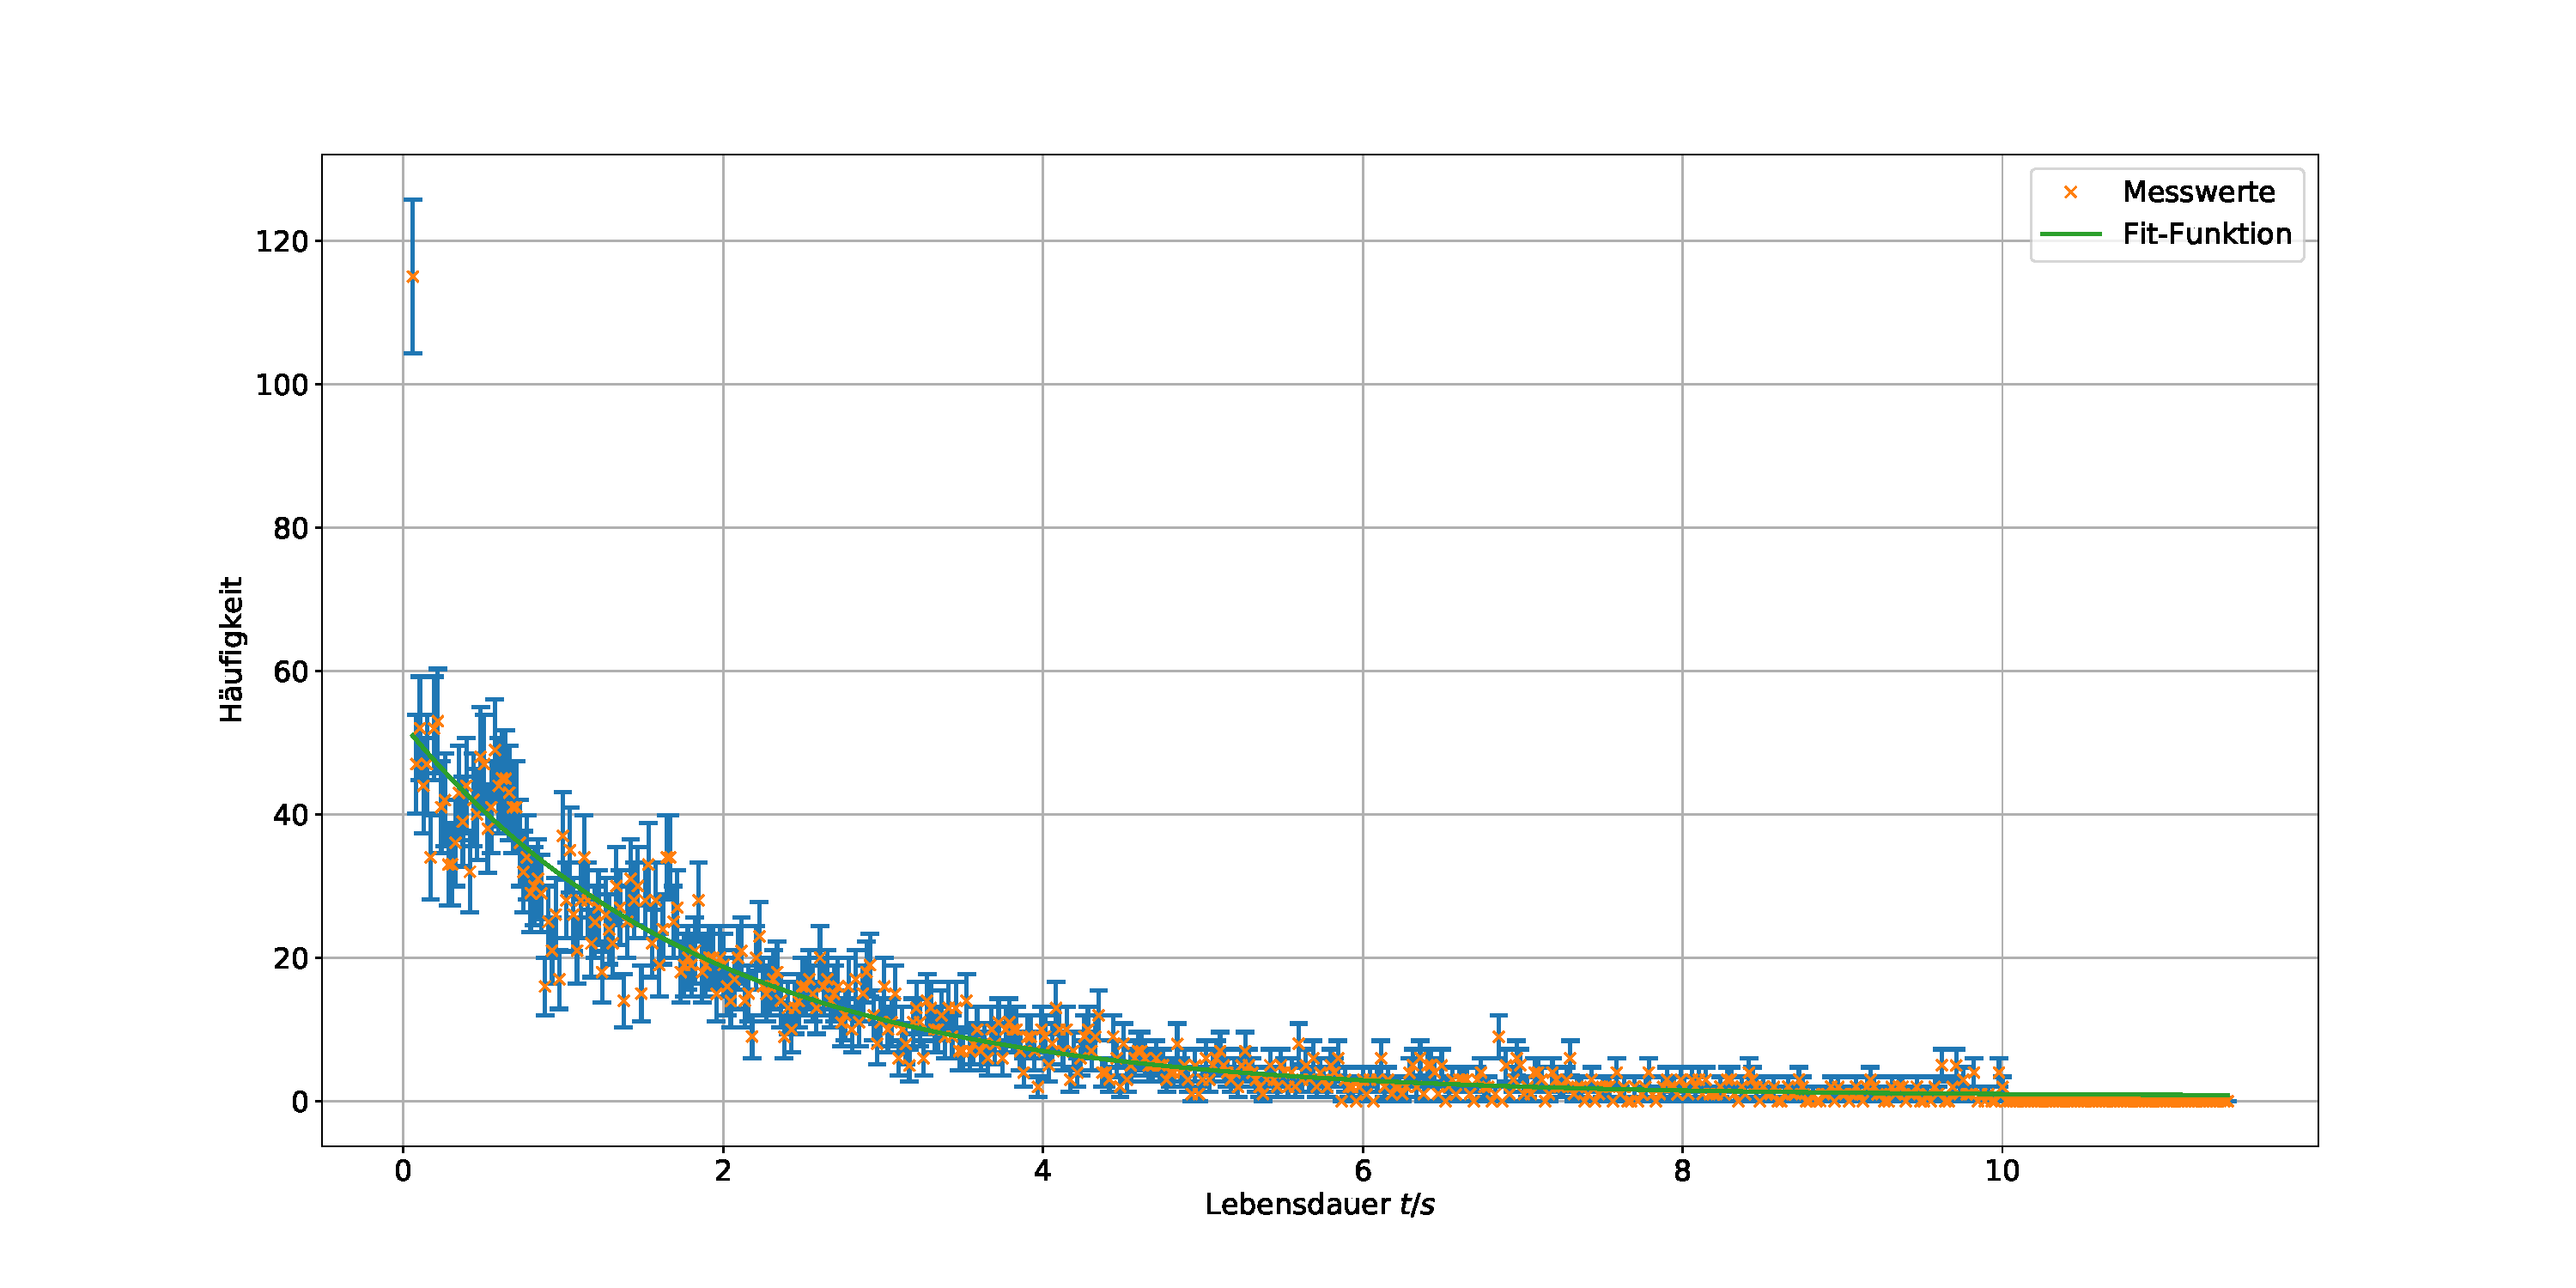
\includegraphics[width=\textwidth]{figmyonen.pdf}
  \caption{Häufigkeit der Myonenzerfälle in Abhängigkeit ihrer Lebensdauer}
  \label{fig:myonen}
\end{figure}
Fit
\begin{equation*}
y = a \exp{(-x b)}+c
\end{equation*}
Fitparameter
\begin{align*}
a  &=&  \SI{51.81005345 \pm 0.9677403}{}\\
b  &=&  \SI{0.52824244 \pm 0.01864355}{}\\
c  &=&  \SI{0.74055349 \pm 0.31446226}{}\\
\end{align*}
\FloatBarrier
